\chapter{Analysis of the dynamics of FH on a BA network}


\section{Introduction}
Since we were more interested in the methodological aspects, and in particular in the capabilities of the FNO, we didn't focus our attention on how the spatial extension of the FH system modifies its dynamics.
In this appendix, we studied how a network of neurons, following the FitzHugh-Nagumo model and linked by diffusion, shows emergent behavior with respect to a single FH neuron. In particular we examined a BA Network of $N=1000$ nodes.

\section{Single Neuron Behavior}
The behavior of a single FH neuron is well-known (it has been described in section \ref{sec:FHN_dynamics}): it can show periodic oscillations, depending on the parameters of the model. 
In particular, we focus on the parameter $I$, which represents an external current applied to the neuron. For certain values of $I$, 
the neuron can exhibit stable limit cycles, leading to periodic firing.

\section{BA Network}
We start by studying a network of $N=1000$ neurons, connected according to the Barabási-Albert (BA) model ($m=2$).
To study the difference between the single neuron and the network, we analyse the output of the potentioal $V$ for the input and the output node.
The main difference is not in the shape of the signal, nor in the critical parameters for which the system starts to oscillate, but in the period of the oscillations.
In fact for a single node the order of the period is always one \footnote{The number of different peaks in the oscillation which we observe in one period}, while for the network
it can be much higher, depending on the parameters of the model and on the structure of the network.




As we can see in figure \ref{fig:periodicity_order_frequency_N=1000_BA}, the frequency of the system has the same transitions from zero as the single neuron, 
but there seems to be other transitions.

To analyze this phenomenon, we can look at the order of the period of the oscillations, which is shown in figure \ref{fig:periodicity_order_N=1000_BA}.
The periodicity Order has been estimated by the number of peaks in one period.
At the transition points (which remain the same as section \ref{sec:FHN_dynamics}) the period exceeds our observation window, so we don't know what really happens: in particular in future investigations we could demonstrate if the period remains finite but large, or if the system manifests even chaotic behavior in these windows
.
\begin{figure}[H]
    \centering
    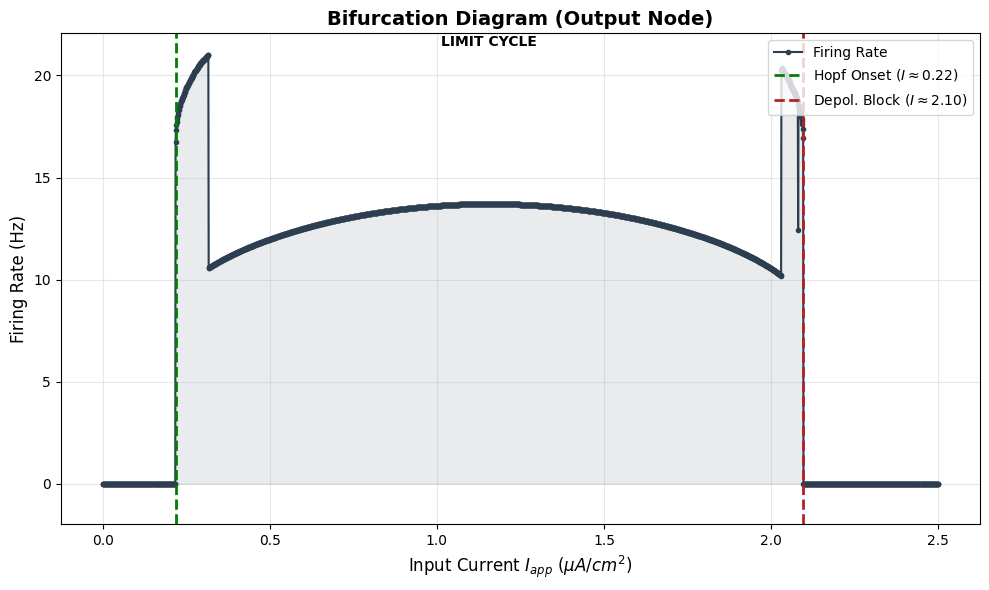
\includegraphics[width=\textwidth]{img/Appendix/Periodicity_Order_BA_N=1000_frequency.png}
    \caption{Frequency Analysis in function of the amplitude of the input current to the system}
    \label{fig:periodicity_order_frequency_N=1000_BA}
\end{figure}




\begin{figure}[H]
    \centering
    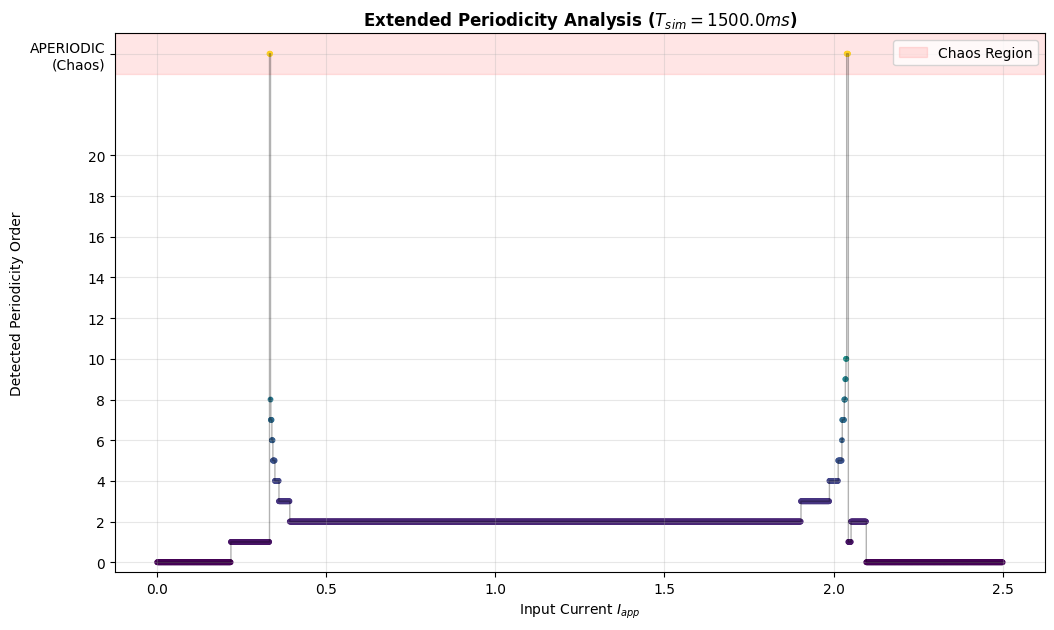
\includegraphics[width=\textwidth]{img/Appendix/Peridiocity_Order_BA_N=100.png}
    \caption{Periodicity Order Analysis in function of the amplitude of the input current to the system}
    \label{fig:periodicity_order_N=100_BA}
\end{figure}



